% ........................................................................... %

A commonly-accepted definition\footnote{\url{http://webservices.xml.com/pub/a/ws/2001/04/04/webservices/index.html} and \url{http://www6.software.ibm.com/developerworks/education/wsbasics/wsbasics-ltr.pdf}} of web services is the following:
\begin{quote}
\textsl{
Web services are a new breed of Web application. They are self-contained, self-describing, modular applications that can be published, located, and invoked across the Web. Web services perform functions, which can be anything from simple requests to complicated business processes... Once a Web service is deployed, other applications (and other Web services) can discover and invoke the deployed service.
}
\end{quote}\

My personal opinion is that this definition is too narrow with the recent advances in technology, and merely applies only to SOAP-based services. Actually, web services are most of the time not just applications of their own. They should rather be considered as \emph{another} presentation-level interface in multi-tiered applications. While in simple cases an application can be created as a sole web service, it is common for elaborated enterprise applications to provide different application communication interfaces to target different types of clients. For example humans will typically interact with the application either through web applications displayed in a browser, or through a desktop application communicating using some communication mean such as Java RMI.\\

We propose another definition of web services that matches our vision of the technology:
\begin{quote}
\textsl{
A web service is an interface of an application that provides programmatic access to other applications through the use of standard web protocols such as HTTP. Data can be exchanged between a service and its requester by using inter-operable, platform-neutral representations such as XML.
}
\end{quote}\

This chapter is organized as follows. We first present application integration of multi-tiered applications and its challenges through the years. We give an overview of the various forms of middleware that facilitate application integration. Finally, we show how web services and the larger services-oriented architectures approach addresses some past and new integration challenges.\\

% ........................................................................... %

\section{Integration: an overview}

% ........................................................................... %

The information system of an organization typically comprises various assets that range from data sources (e.g., relational databases systems) to applications that fulfill different needs (e.g., office tasks suites or business intelligence solutions). Such parts of an information system are either developed ``in-house'' to meet specific requirements, or they are acquired from third-party vendors (with possible customer-specific adaptations). Those assets rarely live isolated to each other. Indeed, it is often necessary for an application to access the data produced by another one, or even to access some parts of an API\footnote{Application Programming Interface} to reuse some of its functionalities.\\

Integrating such assets would be easy in a perfect world where data representation and application interfaces would be uniform. The reality is of course very different as an information system present some of the following sources of heterogeneity:
\begin{itemize}

	\item platforms, including operating systems, hardware architectures and execution platforms
	
	\item databases systems
	
	\item programming languages
	
	\item development techniques and trends.

\end{itemize}
Indeed, as an organization evolves, it will periodically change its technological standards, resulting in the need to  integrate new and legacy systems. For example a warehouse management application may have been developed a few years back using the \emph{Delphi} programming platform while new systems need to be developed in Java. Such legacy systems are often kept ``as-is'' since rewriting them has significant costs (e.g., development and training of employees) for no practical benefit (i.e., the ``old'' application already fulfills the needs). \\

Integration of information systems assets can be performed at different levels as we will briefly see below. We will go through the specific technological details of application integration in the next sections. \\

% ........................................................................... %

\subsection{Data integration}

% ........................................................................... %

\begin{figure}[htbp]
    \centering
    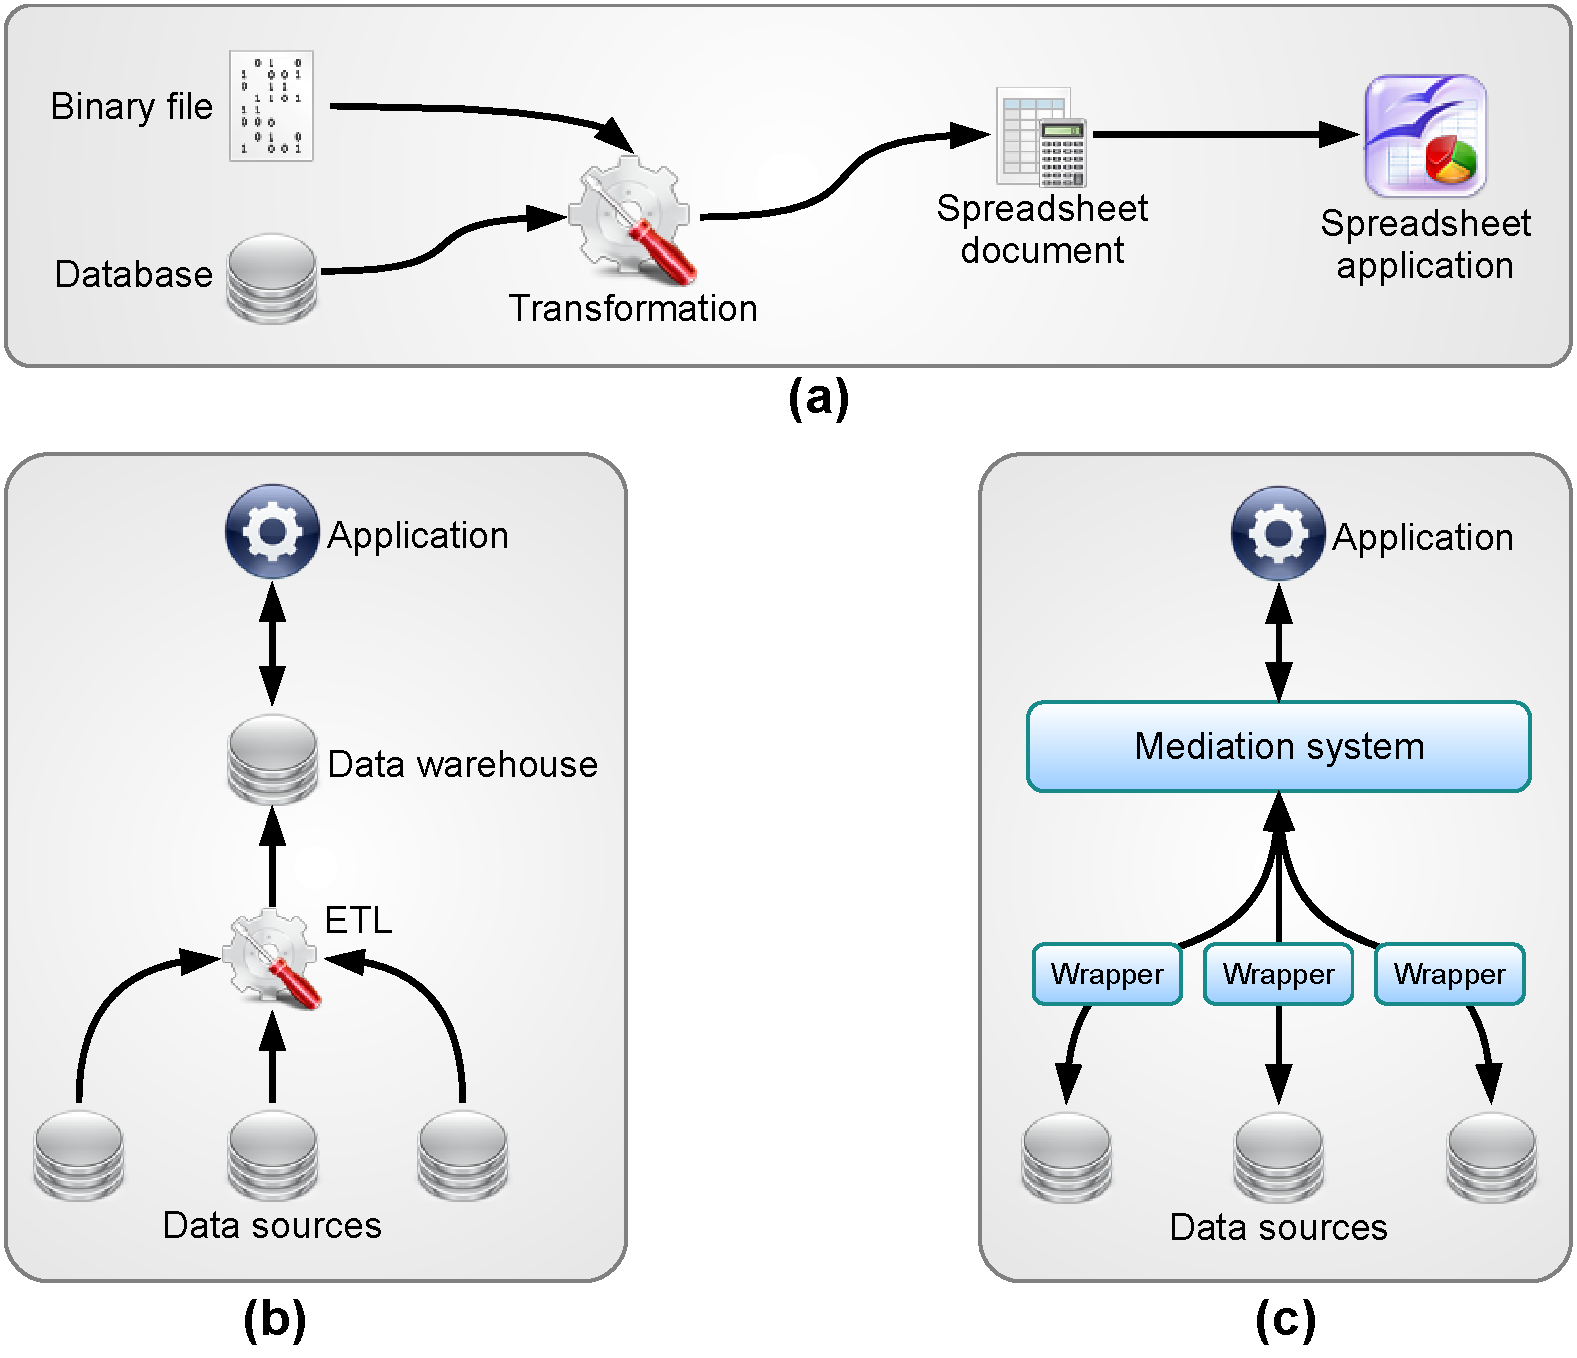
\includegraphics[width=\textwidth]{content/web-services/data-integration}
    \caption{Different approaches for data integration.}
    \label{fig:data-integration}
\end{figure}

Applications physically store their data in files, databases, relational databases and so on. One first approach to data integration is to adapt the data from one or more applications so that another application can process it. An example would be to extract some data from a spreadsheet document and a relational database to pass it to another application that uses both. This typically involves creating ad-hoc transformation components (e.g., scripts or XSLT transformers). The other approach to data integration is to integrate data sources which are generally heterogeneous (and possibly distributed) relational databases. In this case there are two ways of achieving it.
\begin{enumerate}

	\item Materialized approaches use ETL\footnote{Extract, Transform and Load} tools that pull data from several sources, normalize / transform it and finally puts it in \emph{data warehouses}.
	
	\item Virtual approaches use \emph{global-as-view} and \emph{local-as-view} paradigms (or sometimes a mixture of both) where the data is exposed by the mean of queries over the sources (see \cite{Ullman00,Lenzerini02} for an overview and \cite{ChawatheGHPUW94,LevyRO96,LattesR00,HalevyIMMST04} for implementation-related discussions).

\end{enumerate}\

We illustrate these approaches on Figure~\ref{fig:data-integration}. Figure~\ref{fig:data-integration}(a) shows an example of an ad-hoc data transformation where the data is extracted from a binary file and a database, then converted to a spreadsheet document so that end-users can manipulate the data. Figure~\ref{fig:data-integration}(b) illustrates a materialized approach while Figure~\ref{fig:data-integration}(c) shows a virtual approach where the application queries the mediation system like if it was a ``normal'' data source (but the queries are then rewritten to adjust to each source).\\

In practice, ad-hoc transformation components have been widely used so that different applications can share data, or even use data as a direct communication mean. In the case where large data sets are manipulated, or when the data long-term durability is more important than the applications, organizations have been using relational databases rather than custom data formats stored in files (binary, text or XML). At the time of the writing of this document, virtual approaches are still struggling to encompass scalability issues while materialized approaches are mainstream component of information systems. The materialized approaches are relatively well adopted because the very basic idea is to gather and transform data from existing relational databases to be put in another one. This requires both the development of ad-hoc components and frequent processing of the ETL toolchain to refresh the data warehouses. By contrast, virtual approaches promise to facilitate the addition and removal of data sources as well as to provide ``always fresh'' data.\\

% ........................................................................... %

\subsection{Business logic integration}

% ........................................................................... %

Applications can share more than data: they can also share some business logic, either by sharing common pieces of executable software artifacts, or by communicating with each other. Such integration is not new and has always existed under more or less related forms. We give a few examples.\\

\paragraph{Libraries.}
They form reusable sets of data structures, functions and object classes that can be shared by different programs. For example an encryption library falls into this category: several softwares such as a mail user agent, a text processor or a HTTP server can share a thoroughly tested code base rather than re-inventing their own ones. While often limited to the same programming language as they have been developed for, libraries can sometimes be accessed via other languages. This is especially true in the case of platforms such as Java or .Net where several languages can be used in the same application as the platform ultimately provides a language-agnostic runtime virtual machine.\\
  
\paragraph{Components.}
They are a more formalized derivative of libraries. A component is usually a set of object classes providing a self-contained functionality (but components may have dependencies between them).  Using components, applications can be created by assembling as many existing functional units as possible. Ultimately, the final application is just a thin glue code on top of the assembled components. A famous example of component-based system includes the Mozilla\footnote{See \url{http://www.mozilla.org/}} family of softwares. A component is designed to expose an object interface to the client code while the implementation is most of the time completely hidden. In many component technologies, the clients don't even know the programming language that was used for the components implementation. Also, the interface description is usually given in language such as IDL \cite{Lamb87} which is not tied to a given programming language or platform. Some component technologies may also provide life-cycle support for the components by handling their instantiation, configuration and disposal. They may also provide some \emph{services} such as support for logging, authentication, long-term persistence of data or transactional behavior.\\
  
\paragraph{Inter-Process Communications (IPC).}
They are provided by operating systems so that different processes can cooperate. There exist different mechanisms to achieve that: signals, pipes, message-passing calls, shared memory segments or even locks and semaphores are among the range of possibilities to make concurrently running processes communicate with each other, and eventually share some business logic. There are countless examples of applications that work together using those techniques, from low-level communication between a HTTP web server and FastCGI applications to a web browser extension that controls a desktop music player.\\
  
\paragraph{Network-based interfaces.}
They provide a mean for accessing an application over a network and a specific communication protocol on which both parties must agree (i.e., the server and the clients). Providing such an interface is a common pattern in applications. Most relational database management systems provide network interfaces (sometimes also called \emph{listeners}) so that client applications can perform queries and manipulate the data that they store. Another example is the X protocol used in most of the Unix variants and derivatives: it allows both local and remote applications to share a common display. Network-based interfaces allow heterogeneous systems to communicate with each other as long as a common network and communication protocol are agreed.\\
  
\paragraph{Distributed components.}
They are a variant of components where components are not necessarily running along with their client applications. Instead, a client application owns some \emph{stub} code that implement the expected interface, but the actual component implementation is executed on a network-accessible system. The stub code hides the technical details such as the network protocols, resulting in little if no difference to the developer compared to traditional components. \\

% ........................................................................... %

\subsection{Visual presentation integration}

% ........................................................................... %

Beyond data and business logic integration, softwares have also been using integration at the visual presentation layer. As the name suggests, this type of integration aims at assembling existing visual components for creating user interfaces. In turn, each component may be linked with its own (possibly remote) business logic and data source. In some cases, this type of integration can remove the need of performing data or business logic integration work. We give a few examples of visual presentation integration.\\

\paragraph{Application embedding.}
This has been materialized through specification such as OLE or KParts where an application can embed parts of another application. There are countless examples of this such as a web browser embedding a PDF document reader, a word processor embedding a spreadsheet application or a mail user agent embedding a calendar management tool. The embedding can either be simple (e.g., the graphical user interface of one application is put in a frame of the containing application) or more blended (e.g., the embedded application merges some of its own elements such as menu and toolbar items).\\

\paragraph{Graphical interface components.}
The 90's saw the emergence of a market of graphical interface components, mainly due to the rise during this period of time of the so-called \emph{rapid application development} (RAD) environments such as Microsoft Visual Basic or Borland Delphi. They allowed to quickly create applications with a graphical user interface by combining ready-to-use widgets. More elaborated components started to be proposed by third-party vendors, including components without even a visual representation! In fact, the latter components would provide a coarse-grained interface to business logic components, but adding them in a graphical user interface rather than through classical, programmatic calls would be more difficult in light of the average skills of the target developers.\\

\paragraph{Dashboards, web portals.}
Visual dashboards have been provided in a wide-range of contexts, like financial institutions live data monitoring or decisional / business intelligence solutions. The visual components are often specialized to interact with a remote system, either to provide a read-only view of some data, or to provide a mean to interact with it. A modern form of such dashboard systems are web portals often used in intranet systems. Those dashboard / portal systems are often customized depending of the types of end-users. For example a portal will differ for a financial manager and a shipment operator: the former is not interested by data related to the currently delayed shipments while the former does not need the company live market quotations. These systems sometimes allow end-users to re-arrange them. The visual components are generally not isolated from each other and can communicate through events. The way events are dispatched and processed differs greatly depending on the integration technology: each component may send to a central coordinator, or they may be allowed to send events to each other through a message bus.\\

% ........................................................................... %

\section{Multi-tiered applications}

% ........................................................................... %

\begin{figure}[htbp]
    \centering
    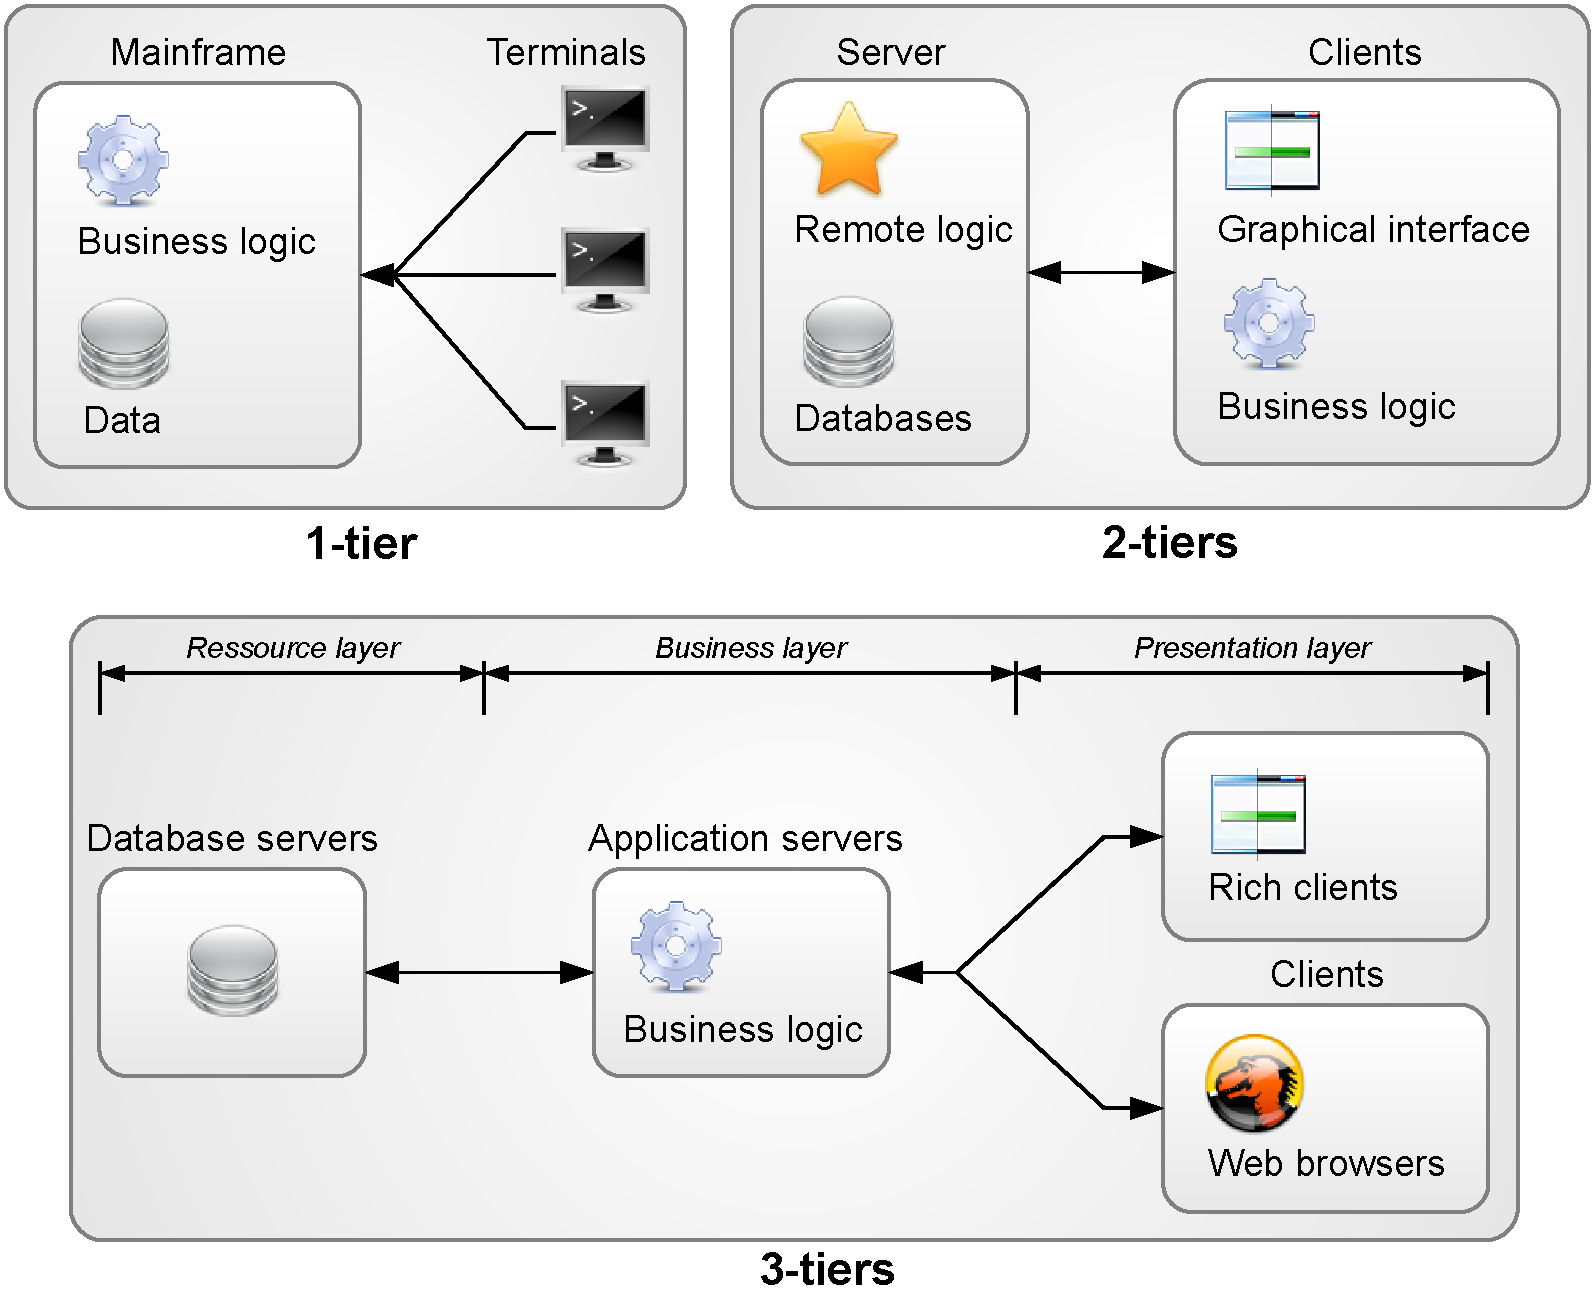
\includegraphics[width=\textwidth]{content/web-services/123-tiers}
    \caption{Overview of typical 1-tier, 2-tiers and 3-tiers architectures.}
    \label{fig:123-tiers}
\end{figure}

The design of enterprise applications has evolved over the years. From an architectural point-of-view, it is common to differentiate different \emph{tiers} of an application. This is especially true with the generalization of distributed applications. We briefly present the typical tiered architectures while an overview of them is available in Figure~\ref{fig:123-tiers}. \\

% ........................................................................... %

\subsection{1-tier (70's -- 80's)}

% ........................................................................... %

This type of architecture is highly reminiscent of the early design of enterprise applications of the 70's and has kept being used throughout many developments of the 80's. Those architectures were relying on applications to be deployed on a single physical machine, called a \emph{mainframe}, while end-users would access it through \emph{terminals} over a network (often a proprietary network solution rather than a standards-based one). A mainframe was typically a powerful and expensive hardware device capable of deploying many applications. In turn, the terminals would be cheap, often console-style devices. This type of architecture turned out to be relatively simple to run with simplified maintenance life-cycles as applications were deployed to a single, central machine. It had however a lot of obvious problems, including the need for expensive hardware upgrades to scale up in the number of concurrent terminals or the single-point of failure syndrome (i.e., several applications become unavailable when the mainframe is down). Those systems were also known to rely on proprietary database management systems when not simply using ad-hoc file hierarchies. Also, most applications would not share common functional units such as data access or concurrency management, although they were deployed on the same machine. Remote access to the applications through applications other than the terminals that were developed on purpose turned out to be an expensive, highly ad-hoc operation. Some techniques have been proposed for adapting the graphical interfaces, either by embedding a terminal emulator or analyzing the textual output to bridge to a more elaborated, modern graphical user interface.\\

% ........................................................................... %

\subsection{2-tiers (90's)}

% ........................................................................... %

This is also called \emph{client / server} in reference to the decomposition of the application units in server-side and client-side units. Those architectures have been primarily pushed forward by the generalization of relational database management systems exposed through network interfaces, thus providing an application neutral way for applications to store and gather data. The database systems are deployed server-side while the remainder of the application (business logic and visual interface) is client-side. There are variants to this: some computation-intensive tasks can be deported to the server as well. Also, some applications could embed client-side databases. A typical example of this is the support of ``offline modes'' where an application needs to store data when no network connection is available and synchronize it with the server when it becomes available again. Compared to 1-tier architectures, 2-tier applications brought a number of improvements, among which the promotion of standard-based networks and normalized data storage and representation systems. Performance-wise, they were also able to introduce clustering of both databases and portions of business logic to handle scalability in the number of clients.\\

% ........................................................................... %

\subsection{3-tiers (end 90's -- 2000's)}

% ........................................................................... %

This type of architecture started to become widespread with the advent of database-driven web applications. It pushed the generalization of \emph{application servers} (e.g., JavaEE, .Net Framework or LAMP\footnote{Acronym for Linux, Apache, MySQL and PHP / Perl / Python (this is not strict as other technologies can be used as replacements).} solutions) that embed the business logic, with the database storage being often delegated to another server. In turn, the presentation layer is accessed through web browsers which are light and generic display devices. Those applications can still be accessed from desktop applications, now called \emph{rich clients} by contrast to web browsers being considered as \emph{thin clients}. Hybrid solutions are often touted under the RIA (Rich Internet Application) acronym that covers a wide-range of solutions such as Adobe Flash, Adobe Flex, Microsoft Silverlight, Mozilla XUL and also to a certain extent Ajax-style web applications. 3-tiers architectures allow hardware requirements to be adjusted given the expected work load of both the application server and the databases. They are relatively easy to cluster for scalability purposes.\\

% ........................................................................... %

\subsection{$n$-tiers}

% ........................................................................... %

\begin{figure}[htbp]
    \centering
    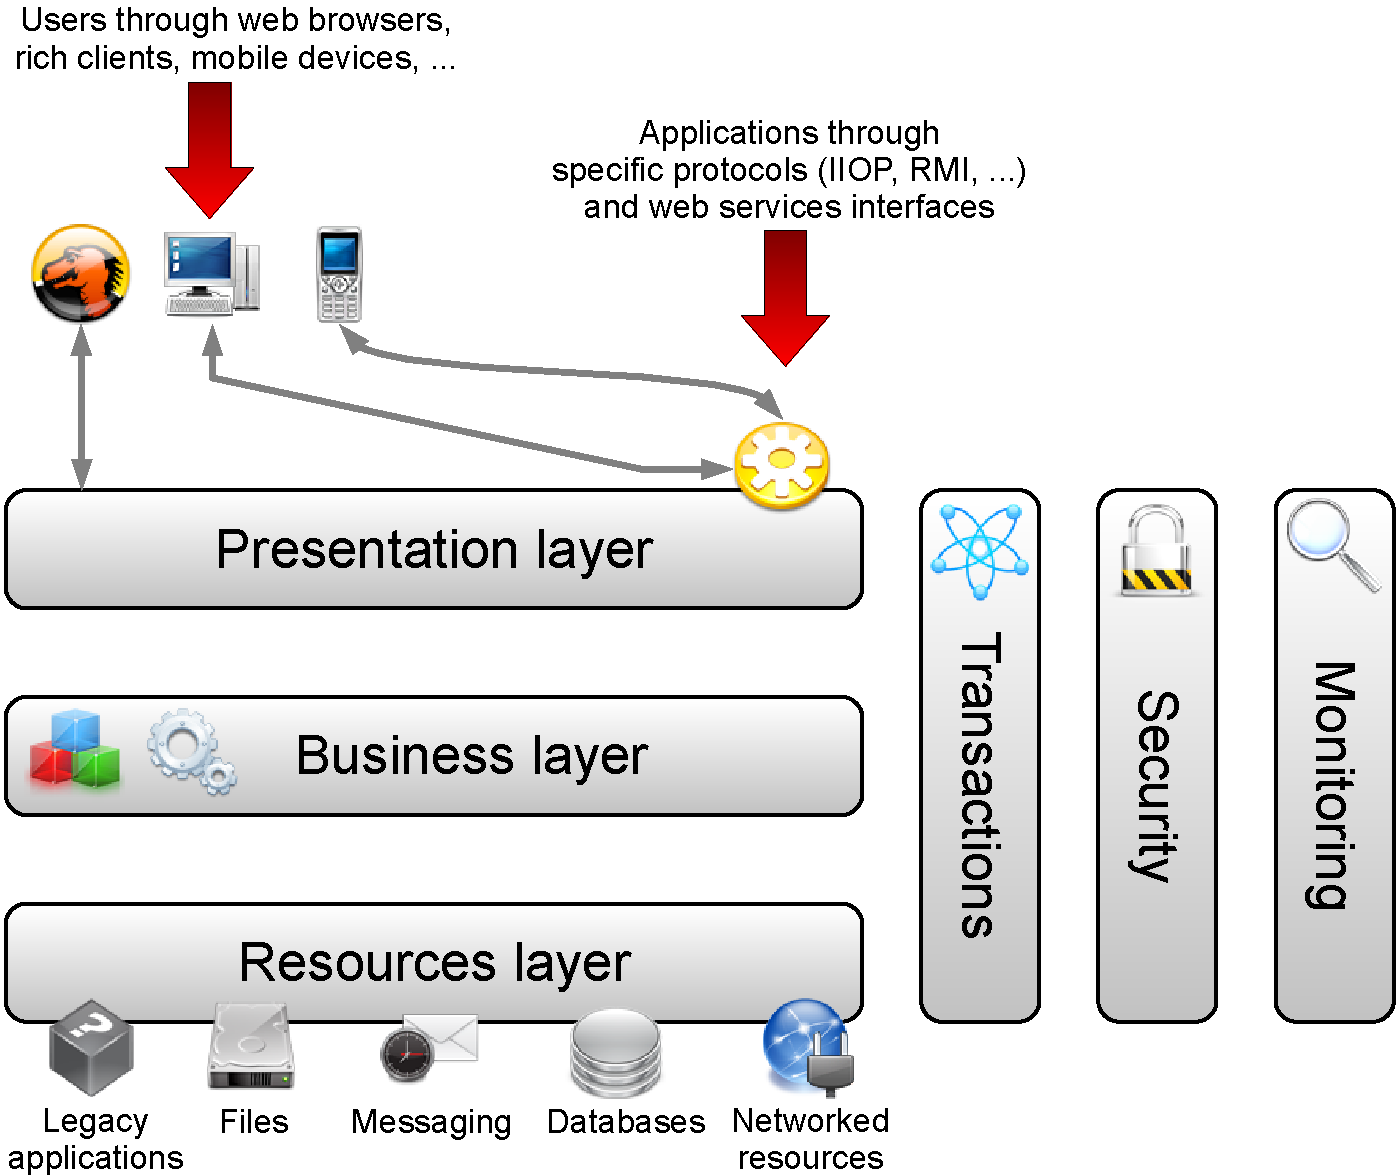
\includegraphics[width=\textwidth]{content/web-services/ntiers-middleware}
    \caption{A typical $n$-tiers architecture.}
    \label{fig:ntiers-middleware}
\end{figure}

$n$-tiers architectures refer to a generalization of 3-tiers architectures to allow a more fine-grained decomposition of the layers of an architecture. We give an example of a $n$-tiers architecture on Figure~\ref{fig:ntiers-middleware}. We can find the ingredients of a 3-tiers architecture.
\begin{itemize}
  
  \item The \emph{resources layer} provides an access to databases, files messaging systems, network interfaces and legacy applications.
  
  \item The \emph{business layer} provides the core functionalities of applications, no matter how they are accessed. This layer typically relies on component technologies (e.g., EJBs\footnote{Enterprise Java Beans}).
  
  \item The \emph{presentation layer} exposes the applications to end-users and applications through a rich set of devices and technologies. In a similar fashion as the model--view--controller paradigm, the very same application can be exposed through different presentation interfaces.
  
\end{itemize}
It should be noted that the presentation layer of a given application eventually exposes an interface that will be accessed through the resources layer of other applications relying on it (this also justifies why we refer to such architectures as $n$-tiers rather than simply 3-tiers). Due to economic constraints, it is often required to reuse an existing (legacy) application: the techniques mostly aim at providing wrappers on top of them, which are part of nothing else but their own presentation layer.\\

Most $n$-tiers platforms rely on the notion of \emph{containers} in every layer. For example, a JavaEE application server provides many of them such as EJB containers, data sources pools (acting as containers) or web applications containers. The purpose of having containers is twofold.
\begin{enumerate}
  
  \item Handle the life-cycle of resources. For example an EJB component doesn't have to manage its instantiation of configuration, nor its clients do: the container does that for them.
  
  \item Provide services to the resources that the containers manage.
  
\end{enumerate}\

In terms of services, we have presented three typical ones on Figure~\ref{fig:ntiers-middleware}. They are cross-cutting concerns as the different layers require such services, albeit with different implementations due to each layer specificities. For example transaction support is different for distributed component objects in the business layer and relational database management systems. Security comprises both \emph{authentication} (e.g., a container checks that a client has enough credential to access a managed resource such as an EJB component) and \emph{confidentiality} (e.g., the remote invocation of an EJB component is performed over an encrypted network protocol). Finally, monitoring is an essential part in $n$-tiers systems as they are typically distributed and accessed by many concurrent clients. Indeed, it allows the inspection of logs to report failures or discover and analyze how the application is used in practice. It also allows measuring the performance of each component that is involved in the application. \\

Like in the case of 3-tiers architectures, $n$-tiers architectures allow fine sizing of the hardware requirements to run the applications. They also allow elaborated topologies to be used to improve scalability and availability of the applications. For instance a clustered application server can transparently handle the failure of one node by ensuring that the other nodes also have a copy of the session of a client, thus ensuring that the client requests can still be processed after the node is unavailable (e.g., failure or maintenance upgrades).\\

% ........................................................................... %

\section{Application integration middlewares}

% ........................................................................... %

Getting back on Figure~\ref{fig:ntiers-middleware}, there is something that we (intentionally) did not explain: \textit{how can one layer interact with one that is above, below or beside it?}
%
This is all done through software gluing tools and components called \emph{middlewares}. A more formal definition would be the following one.\\

\begin{definition}
A middleware allows connecting software components and applications.
\end{definition}

The role of a middleware goes beyond just bridging heterogeneous software artifacts: it hides some of their inherent complexity (much like a \emph{Facade} does in object-oriented programming). A middleware can provide some development-time infrastructure (e.g., developer tools) or runtime infrastructure (e.g., deployed execution and monitoring components). They can of course also provide both. We give a few examples of middlewares families.

\begin{description}
  
  \item[Remote procedure calls (RPC)] (or their object variants often referred to as \emph{remote method invocations} -- RMI) will be detailed below.
  
  \item[Object request brokers (ORB)] allow clients to delegate the discovery and binding processes of a component that matches a given programmatic interface. The broker will select the best component according to the criteria it has been configured for, and will provide the clients with objects without them knowing what the concrete implementation is. To do that, an ORB relies on directories of components. Corba (\url{http://www.corba.org/}) is an example of a middleware comprising ORB technology.
  
  \item[Message-oriented middlewares (MOM)] will be detailed below.
  
  \item[Data access frameworks and relational-object mappers] are examples of middlewares that decouple the business and the resources layers. By using them, the business layer of an application has a uniform way of accessing databases, no matter their vendors and their configuration details such as the network protocol and server location. Examples of data access frameworks include ODBC or JDBC that define standardized programmatic interfaces for accessing heterogeneous database systems. Relational-object mappers also reduce the complexity of passing the data between a relational model and an object model, for example ultimately hiding from the business logic layer the fact that a relational database is being manipulated underneath. Examples of such systems include the Java Persistence API (JPA) or the Hibernate framework.
  
  \item[Distributed database systems] allow different servers to be connected with each other. This allows to transparently perform queries over local and remote tables. This can be sometimes used for integrating heterogeneous data sources. However, very few systems support such a feature (e.g., Oracle Database Server) and inter-operability is limited to the same vendor unless specific network protocol adapters are developed.
  
  \item[Transaction monitors (TP)] ensure the coordination of distributed components as part of a transactional process. Relational database management systems have typically efficient support for transactions on data manipulation, hence it is often natural to rely on them for transactional behavior of applications. This is however not always possible when different business logic components have to be assembled as each of them may not ultimately rely on the same databases. Those systems usually implement variants of the three-phases commit protocol \cite{SkeenS83}. An example TP is the Java Transactional API (JTA).
  
  \item[Workflow management systems and rule engines] are both examples of middlewares that associate end-users in the application. Workflow systems allow designing applications by orchestrating self-contained components and tasks. End-users can be implicated in the process (e.g., an accountant that validates a purchase order), or in the workflow design (e.g., business analysts). Rule engines allow certain decisions to be made by a system based on a set of facts. A decision leads to an application component to be leveraged (e.g., a purchase order is sent to the accounting application and to the delivery planning system). The facts are generally expressed in a way that domain-experts (which are rarely software development savy!) can add, edit or remove them. Examples of such systems include JBoss Rules (formerly Drools) or JBoss jBPM.
  
\end{description}\

The platforms that are based on middleware technologies rarely support only a single family of them. Full-stack application servers such as the ones that implement the JavaEE specification implement much of the ones mentioned above.\\

RPC and MOM style middlewares are of special interest in the case of web services. We present them hereafter.\\

% ........................................................................... %

\subsection{RPC-style middlewares}

% ........................................................................... %

\begin{figure}[htbp]
    \centering
    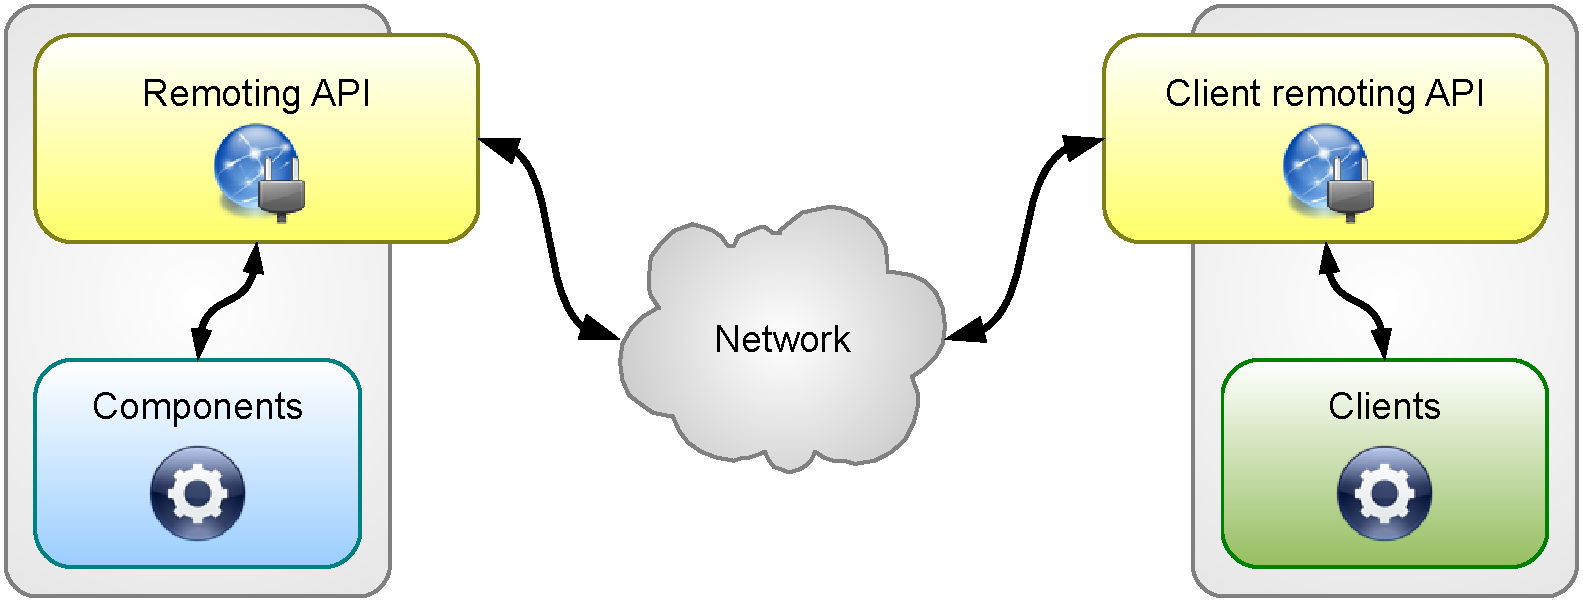
\includegraphics[width=\textwidth]{content/web-services/rpc-middleware}
    \caption{RPC-style middleware.}
    \label{fig:rpc-middleware}
\end{figure}

Remote procedure calls (RPC) middlewares allow applications to communicate through regular \emph{procedure / function / method} calls of programming languages. Such a call looks like a normal, local invocation of some application code, but in reality, the actual code that is executed runs on a remote machine. To do that, RPC middlewares encode the call parameters in a message that is sent over the network to the remote machine that will run the actual code. Once it has been executed, a response message is sent back to the invoking application with a return valued being encoded inside. An illustration is provided on Figure~\ref{fig:rpc-middleware}. \\

The preparation of the message (either for performing the call or returning the value) is called \emph{marshaling}. Similarly, the decoding of the message (either on the remote server or the invoker side) is called \emph{unmarshaling}. The terminology may also differ as in some technologies, the terms \emph{serialization} and \emph{de-serialization} are used instead. While most RPC middlewares use their own message encoding schemes (either binary or text based), standard representations such as \emph{ASN.1} can be used.\\

RCP middlewares have been implemented in a lot of languages and platforms. Examples include distributed components such as EJBs (remote session beans) or Microsoft DCOM. These middlewares are generally well appreciated by developers as they don't require a significant paradigm shift (i.e., they still use regular procedure invocations). Interoperability is possible between different languages and platforms as long as compatible client and server libraries exist. Another particularity of RPC middlewares is that they provide synchronous communications between distributed systems, although asynchronous handling of invocations is possible in some frameworks using \emph{callback functions}.\\

% ........................................................................... %

\subsection{MOM-style middlewares}

% ........................................................................... %

\begin{figure}[htbp]
    \centering
    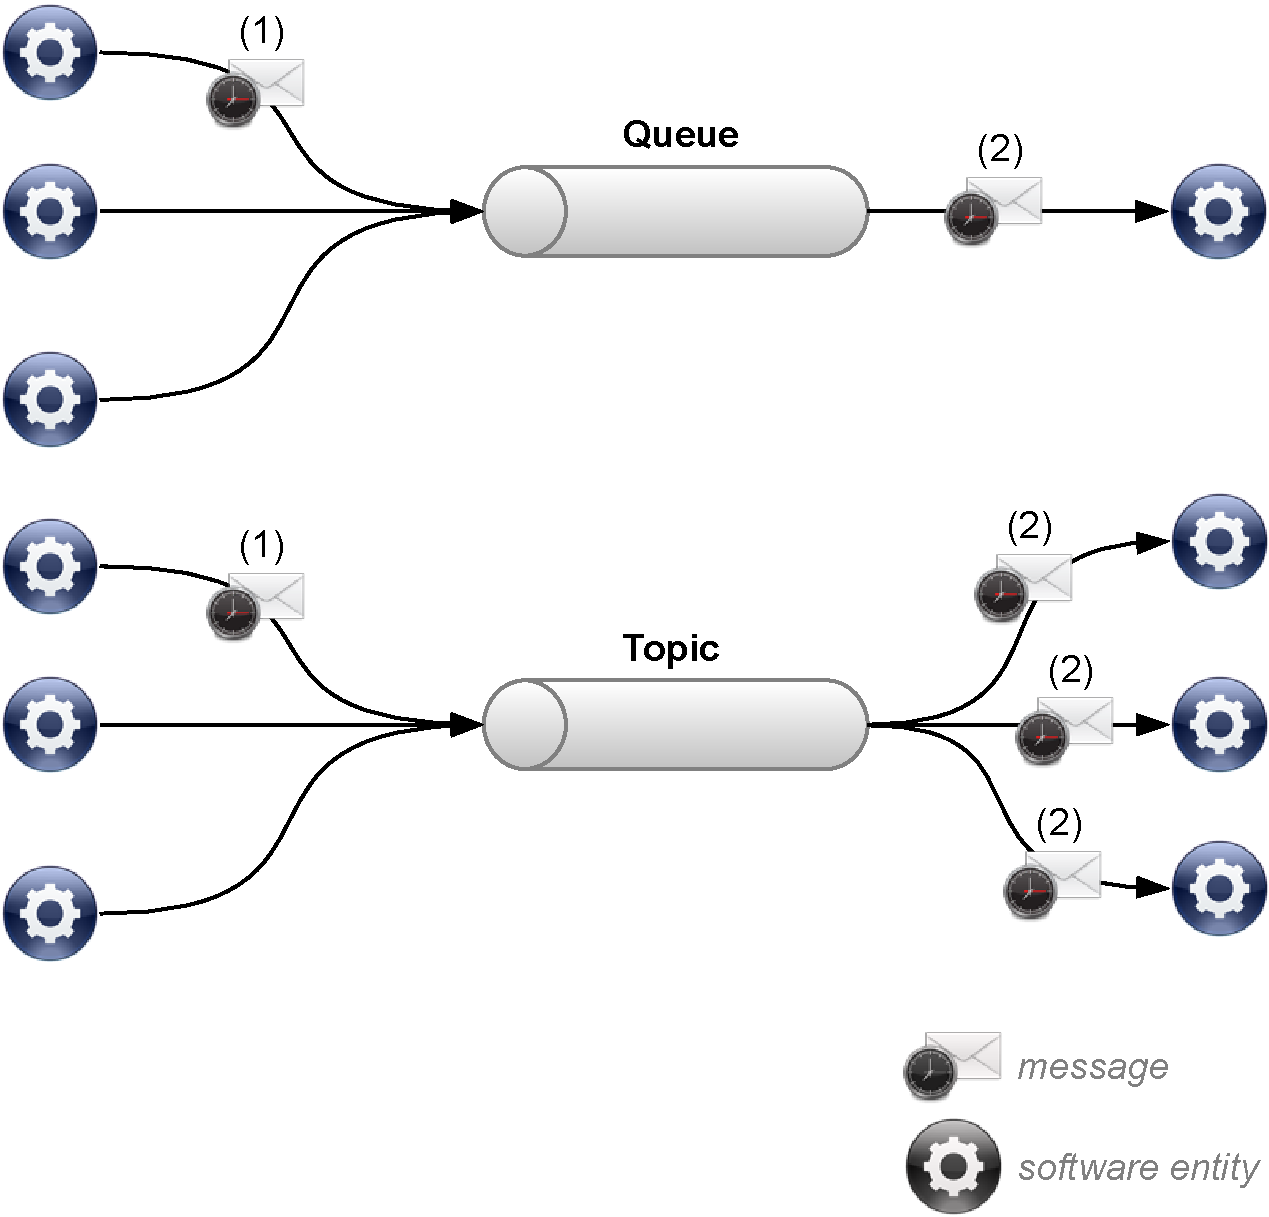
\includegraphics[width=\textwidth]{content/web-services/messaging-middleware}
    \caption{Messaging middleware.}
    \label{fig:messaging-middleware}
\end{figure}

Message-oriented middlewares (MOM) allow the communication between applications through (mostly asynchronous) messages. By contrast to RPC middlewares, the messages do not cary ``function call'' semantics as they are rather general purpose documents exchanged between the systems. A MOM is responsible for collecting and routing messages. It also ensures their integrity and that the messages are not being lost. Quality of service requirements are generally available, with priorities and validity expiration dates being the two most commonly used ones. A MOM is also able to transform the messages contents. This is useful when a message needs to be routed to an application that does not understand the initial message data format. To do this, either ad-hoc scripts and software routines can be used, or declarative approaches can be leveraged (e.g., XSLT to transform XML documents from one dialect to another one).\\

MOM allow heterogeneous systems to easily communicate as long as network protocols and data formats are agreed. The asynchronous nature of the communications allow the support of long-running business processes (e.g., a provisioning process may span for a few weeks from the beginning to the end of the operations). This also allows great scalability to be achieved under sporadic peak loads: a MOM guarantees data delivery (they cannot be lost) and critical messages may still be handled rapidly compared to lower priority messages that can be re-scheduled later. This asynchronous nature of the communications is however sometimes less natural than RPC for developers, and the testing of the systems may require more attention to be done properly.\\

Two message atomic communication patterns are found in MOM (see Figure~\ref{fig:messaging-middleware}). More elaborated schemes can be defined based on those ones. The first one is the \emph{message queue} that provides a $n$-to-$1$ communication between $n$ message emitters and one receiver. The second one is the \emph{message topic} that allows broadcasting messages between $n$ emitters and $m$ receivers. In this pattern, $m$ receivers have subscribed to the \emph{topic} and when any of the $n$ emitters sends a message, all of them will receive it. An example specification of a MOM is the Java Messaging System (JMS).\\

Message-oriented middleware is an essential ingredient of application integration technologies like the so-called ``enterprise services buses'' (ESBs). Indeed, they provide a loose-coupling between the systems as the messages data is language and platform agnostic (this is less often the case with RPC middlewares because of the ``function call'' semantics).\\

% ........................................................................... %

\subsection{Application integration example}

% ........................................................................... %

\begin{figure}[htbp]
    \centering
    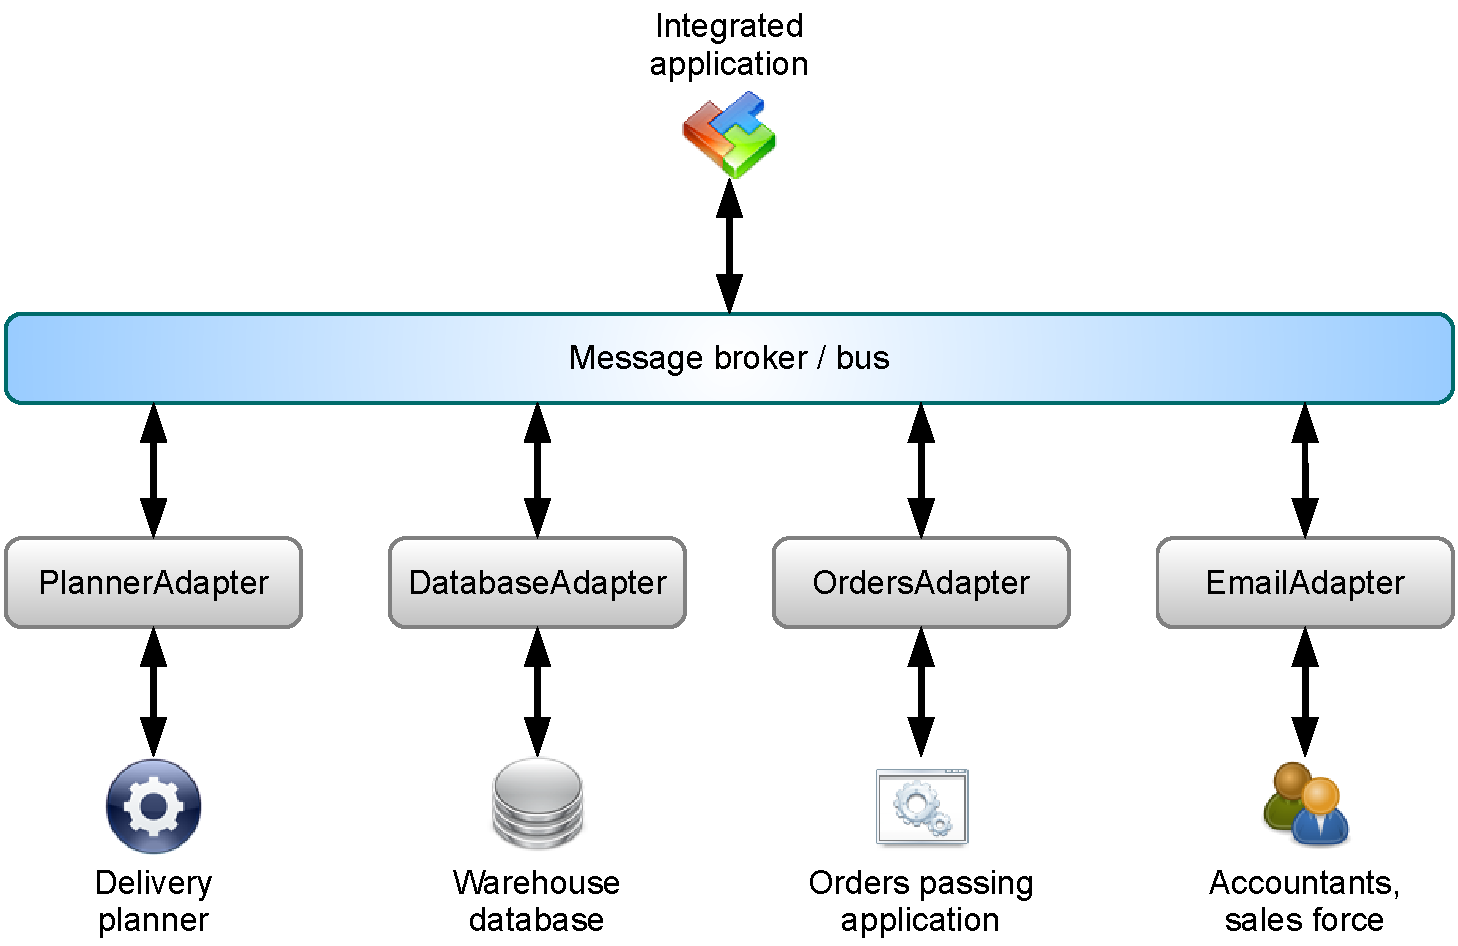
\includegraphics[width=\textwidth]{content/web-services/eai-scenario}
    \caption{Enterprise application integration using a message broker / bus.}
    \label{fig:eai-scenario}
\end{figure}

We give an example of MOM-based application integration on Figure~\ref{fig:eai-scenario}. In this example, several components are connected on a message bus (a generic term to denote a set of queues and topics that route messages between the components). The integration creates a composite, integrated application that handles the whole business process of the purchase orders management, from the order to the delivery.
\begin{enumerate}
  
  \item A delivery planner component computes the next day deliveries of the goods.
  
  \item A warehouse database owns the information of the available goods.
  
  \item An order-passing application is manipulated by the sales team to order goods asked by customers.
  
  \item Accountants and the sales team are part of the process.
  
\end{enumerate}
Each component is plugged onto the message bus through an \emph{adapter} whose role is to bridge between the bus and the component. For example, the \emph{EmailAdapter} is able to send an email to the accountants when notified from a message sent over the bus that an order has been passed. Please note that each adapter may in turn require a middleware technology (e.g., the \emph{DeliveryPlanner} component may be accessed through a RPC API).\\

A typical messages flow of such a business process may be the following:
\begin{enumerate}
  
  \item check for the availability of some goods: \emph{OrdersAdapter} sends a message to the \emph{availability} queue on which \emph{DatabaseAdapter} is the processing entity, which in turns sends back a reply
  
  \item purchase initiation: \emph{OrdersAdapter} sends a purchase order message to the \emph{purchase} topic on which \emph{EmailAdapter} and \emph{DatabaseAdapter} have subscribed, resulting in the goods being locked in the warehouse and an email sent to the accountants
  
  \item purchase validation by the accountants: \emph{EmailAdapter} sends a message to the \emph{validated-purchases} topic where \emph{DatabaseAdapter} and \emph{DeliveryAdapter} have subscribed, resulting in the goods to be removed from the warehouse and a delivery being planed
  
  \item delivery confirmation: \emph{DeliveryAdapter} sends a delivery confirmation to the \emph{delivery-confirmations} queue whose handler is \emph{EmailAdapter}, resulting in the sales force team being notified by email of the goods delivery date, in turn having them notifying the customer (either by email of phone call).
  
\end{enumerate}\

It is interesting to note that the components are really loosely coupled: at no point they know the real software entity they are talking as the MOM takes care of the routing logic. All a component needs to know is the messages data formats, which resources it needs to be the handler of (or which topics it must subscribe to) and which resources (queues or topics) the messages need to be sent to. This allows replacing one component by another one. \\

Application integration is a complex domain that requires high architectural and technical skills. We refer the reader to \cite{EAA02} for a good understanding of the domain.\\

% ........................................................................... %

\section{Web services interface technologies}

% ........................................................................... %

We now give an overview of the current web services technologies which form a new type of presentation layer interfaces for accessing applications. As we will see, each technology has its preferred use cases. While overlaps exist (e.g., SOAP versus REST), these technologies should be considered as complementary rather than competing.\\

% ........................................................................... %

\subsection{XML-RPC}

% ........................................................................... %

\begin{table}[htbp]
\centering
\begin{tabular}{| p{0.2\textwidth} | p{0.65\textwidth} |}

\hline

\textbf{Type name} & \textbf{Description} \\ \hline

\texttt{boolean} & Boolean values. \\ \hline

\texttt{integer} & Integer values. \\ \hline

\texttt{double} & Floating-point numbers, double precision. \\ \hline

\texttt{string} & Characters strings. \\ \hline

\texttt{date time} & Date / time values, specified using the ISO 8601 standard. \\ \hline

\texttt{array} & Array of heterogeneous XML-RPC data types. \\ \hline

\texttt{struct} & Similar to the structures of programming languages such as C or Pascal. It is essentially a map data structure. \\ \hline

\texttt{base64} & Allows to encode as \emph{base64} text any kind of binary data, or when no other data type suits the need. A typical example is to attach a media document to a request or response. \\ \hline

\end{tabular}
\caption{XML-RPC data types.}
\label{tab:xmlrpc-datatypes}
\end{table}

XML-RPC is the first form of web services to have appeared. Defined in \cite{DW98}, it is a small and simple specification for performing RPC-style communications between systems. As the name suggests, the marshaling and unmarshaling of the invocations are done using XML as the data encoding mean. The marshaled messages are conveyed using the HTTP protocol (HTTPS can be used for secure point-to-point communications).\\

XML-RPC messages exchanged between a requester and a provider can be of three types. The first one is a \emph{method call} sent by the requester, where the message contains a name for the RPC method to be called, and the parameters with their names and values. In turn, the provider can return a \emph{method response} which consists of several ordered parameters and their corresponding values. In case the provider cannot properly handle a method call (for instance the method name doesn't exist, or the parameters values are wrong), a \emph{fault} is returned as a value of the method response. We provide here sample XML-RPC messages of a service that would compute the sum of 2 integers $a$ and $b$. A typical request with $a = 1$ and $b = 2$ would be:
\verbatiminput{content/web-services/xmlrpc-request.xml}
and the response would be:
\verbatiminput{content/web-services/xmlrpc-response.xml}
In case the requester assigns a string to $a$ such as $a = "\mbox{\texttt{plop}}"$, then the response would be a fault such as:
\verbatiminput{content/web-services/xmlrpc-fault.xml} \

Both the limited data types (see Table~\ref{tab:xmlrpc-datatypes}) and the general minimalism in XML-RPC have facilitated its widespread adoption. Most programming languages and platforms have some support for XML-RPC. What's more, the level of inter-operability between server and client libraries is excellent. It has however a few limitation: the set of data types may be too limited in some cases, sending binary documents (e.g., pictures) requires \emph{base64} encoding and performing large requests can have a significant performance hit.

% ........................................................................... %

\subsection{SOAP}

% ........................................................................... %

SOAP \cite{MGMH+03} is a standard protocol defined by the W3C for exchanging XML-based messages between web services and their requesters. It builds on top of widespread existing standards such as XML, URI, HTTP or SMTP. Basically, a SOAP message is an XML document that acts as an envelope for the content being sent. In turn, a SOAP message is meant to be transported over various kind of protocols, the most used being HTTP / HTTPS. While the usual expected alternative is the \emph{Standard Mail Transfer Protocol} (SMTP), real-world applications have been using IIOP (from Corba), XMPP (Jabber open instant messaging) or even JMS (\emph{Java Messaging System}) to route SOAP messages.\\

\begin{figure}[htbp]
    \centering
    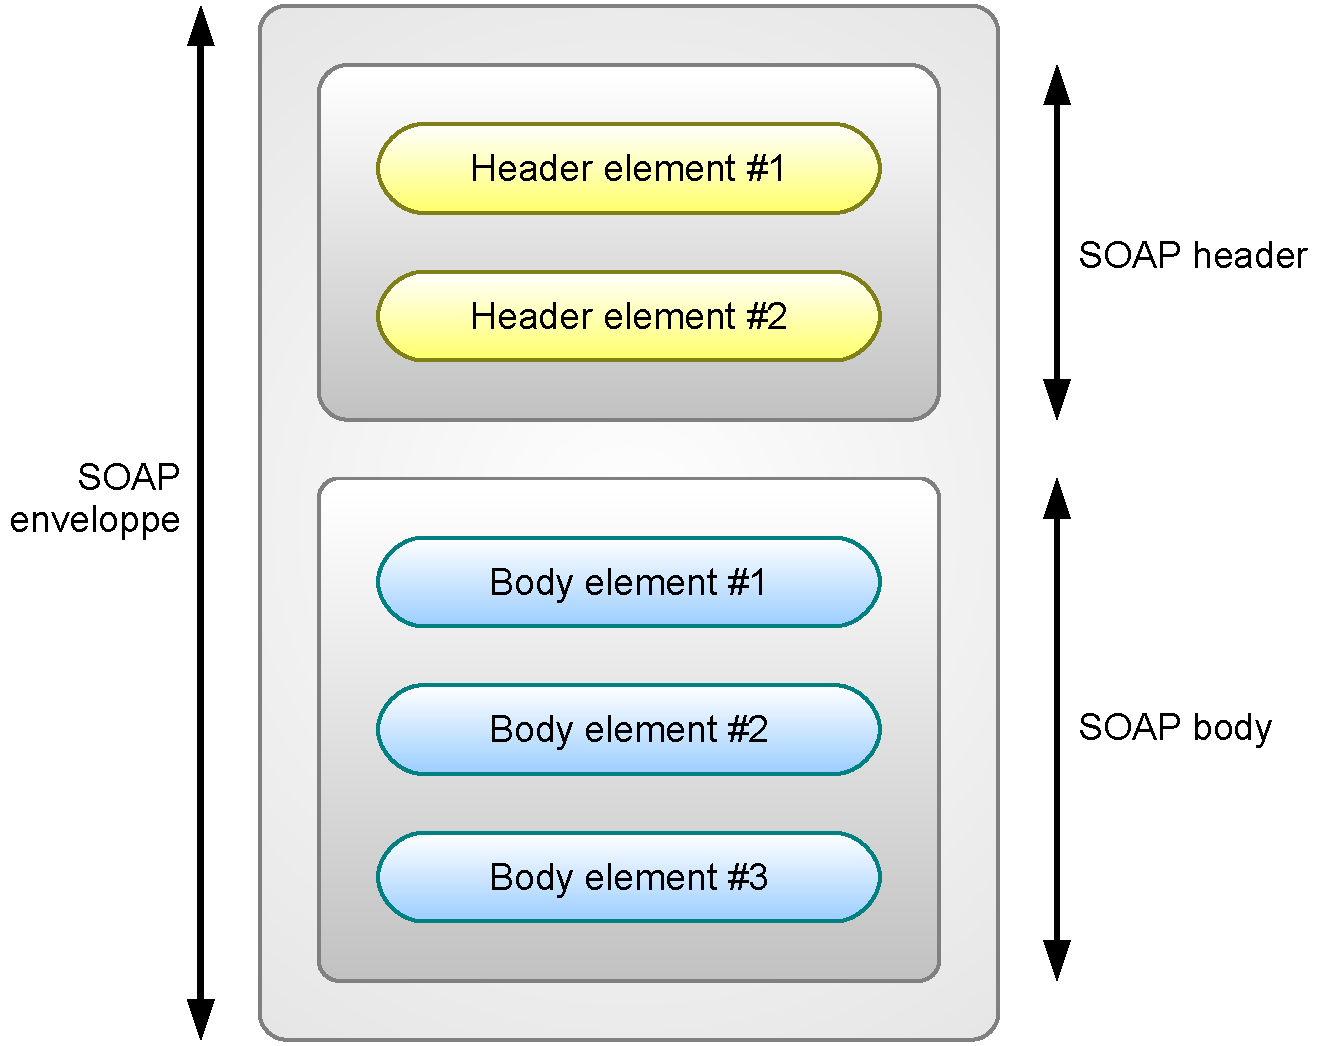
\includegraphics[width=\textwidth]{content/web-services/soap-structure}
    \caption{Structure of a SOAP message.}
    \label{fig:soap-structure}
\end{figure}

Figure~\ref{fig:soap-structure} shows the structure of a SOAP message. The envelope contains two main sections that we describe hereafter.
\begin{enumerate}

    \item \emph{The header} can contain any number of XML elements that contain useful information attached to the message. This can include addressing informations, transaction reference identifiers, quality of service requirements and so on.
    
    \item \emph{The body} contains the actual data to be transported in the SOAP message. This can be any number of XML elements, which can in turn be full XML documents of their own. In case the service that emits the message encounters some form of error, the body will contain a \emph{fault section}, whose structure and semantics have been normatively defined in the SOAP specification.

\end{enumerate}\

We give here an example SOAP message exchanged between a fictional travel agency service and its requester\footnote{The example is from the \emph{SOAP Primer} at \url{http://www.w3.org/TR/soap12-part0/}}:
{\footnotesize \verbatiminput{content/web-services/soap-message.xml}}
We can see that the different pieces of information of the message are cleanly separated by the use of XML namespaces. SOAP owns its own namespace (\url{http://www.w3.org/2003/05/soap-envelope}), while the various header elements use application-specific ones and so do the body elements. The first part of the body element contains information about the desired flight departure and return informations, while the second is related to lodging. The header shows many useful informations attached to the message, such as a reference identifier, the date the message has been issued, or the passenger reference. It should be noted that SOAP messages can be routed through several SOAP-aware nodes, and they can consume and add headers on the way for processing purposes.\\

SOAP messages can be used either to simulate RCP-style communications, or document-style communications which are similar to messaging systems such as JMS. SOAP was actually built with the idea of being the successor of XML-RPC, hence this style of communication was prevalent over document-style until recently. SOAP provides 3 main kinds of body data encoding styles.
\begin{enumerate}

    \item \emph{RPC encoding}: as the name suggests, it is used for encoding RPC-style communication parameters. The way the \emph{procedure} name, \emph{parameter} names and values, or \emph{return} values are encoded in the body of the SOAP message is standardized in the SOAP specification.
    
    \item \emph{RPC encoding literal}: this is also used to mimic RPC-style communications, however the RPC informations encoding is freeform and defined by the service developers.
    
    \item \emph{Document-style}: this is used for messaging-style communications, and the content of the SOAP body is freeform.

\end{enumerate}\

The \emph{Web Services Description Language} (WSDL) \cite{ECFC+01} is an important building block of SOAP-based web services. It provides a description of the static interface of a SOAP-based web service. As such, it specifies the operations supported by the service, the data schemas, and the binding information used to communicate with the service such as the transport protocol being used (ex: HTTP) and the location of the service (in the case of HTTP as a transport protocol, a URL). The following is an example WSDL document taken from \url{http://www.w3.org/TR/wsdl}:
{\footnotesize \verbatiminput{content/web-services/wsdl.xml}}
We outline briefly the content of the document. The \emph{types} section specifies the data types that can be used in the SOAP documents to be exchanged with the service. Their specification is done using XML Schema (\url{http://www.w3.org/XML/Schema}). The \emph{message} elements define the actual messages types, by referring to the data types above. The \emph{portType} define abstract endpoints for exchanging messages with the service, while the \emph{binding} specifies how to technically transmit those messages to the endpoints. Finally, the \emph{service} element binds the ports to their location, for example URLs.\\

A WSDL document can be used to bind to a SOAP-based service in two ways: either client invocation source code can be generated from the WSDL, or the binding can be performed dynamically at runtime. The latter case is especially possible with dynamic and reflexive languages such as \emph{Java} or \emph{Ruby}, by using the \emph{Proxy} design-pattern \cite{Gamma95}. Once either the static or dynamic binding has been performed, the service can be invoked. WSDL documents can be published to be discovered dynamically by clients. To do that, the \emph{Universal Description, Discovery and Integration (UDDI) protocol} (see \url{http://www.uddi.org/}) provides a way for repositories to contain service functional and non-functional descriptions. Ultimately, a client interested in a given discovered service is able to obtain its WSDL description and bind to it.\\

Several specifications are gravitating around the SOAP web services stack \cite{HMBBFC+06}. Most of them are actually irrelevant with no practical adoption in real-world use-cases \cite{WS-standards}. Among the very few relevant ones we have:
\begin{itemize}
  
  \item WS-Security (\url{http://docs.oasis-open.org/wss/v1.1/}), a specification for end-to-end preservation of the messages confidentiality and authenticity
  
  \item WS-Addressing (\url{http://www.w3.org/Submission/ws-addressing/}), which defines a standard representation for endpoint references and routing schemes (useful for correlation in stateful web services)
  
  \item WS-Policy (\url{http://www.w3.org/Submission/WS-Policy/}), a standard representation of quality of service requirements (e.g., security, message-encoding optimizations, ...)
  
  \item WS-Reliability (\url{http://docs.oasis-open.org/wsrm/ws-reliability/v1.1}) is useful for ensuring that messages are properly delivered in contexts that are not point-to-point communications between the service provider and its requesters
  
  \item WS-Coordination (\url{http://docs.oasis-open.org/ws-tx/wscoor/2006/06/}) and WS-Transaction (\url{http://dev2dev.bea.com/pub/a/2004/01/ws-transaction.html}) allow the coordination of web services.
  
\end{itemize}\

SOAP-based web services support rich XML documents as well as elaborated message exchange patterns that go beyond the classic ``request / response'' pattern. It has however a few limitations. For instance it is complicated to send non-XML data (e.g., binary content) through SOAP messages. There is a W3C proposal for this purpose: \emph{SOAP messages with attachments} (\url{http://www.w3.org/TR/SOAP-attachments}) but it only works when HTTP(S) is used as the transport protocol. Another common critique among developers is that most tools and framework encourage a bottom-up approach to web services development (i.e., starting from code then having web services artifacts such as WSDL documents being generated automatically). This approach limits long-term stability of a SOAP-based interface (e.g., a minor change in the implementation class may break the WSDL interface contract). Also, many tools promote too much reliance on the generation of client-side proxy code rather than encouraging dynamic invocations, leading the code to be generated every time a change as little as the endpoint IP address changes. Finally, support of SOAP in libraries and framework greatly differs in terms of inter-operability. This lead to the creation of the \emph{WS-I Basic Profile} (\url{http://www.ws-i.org/Profiles/BasicProfile-1.0.html}) to clarify the SOAP and WSDL standards and define a set of rules for SOAP server and client libraries to be inter-operable.\\

% ........................................................................... %

\subsection{REST}

% ........................................................................... %

The concept of REST\footnote{REST stands for \emph{\textbf{RE}presentational \textbf{S}tate of \textbf{T}ransfer}.}-style services first appeared in \cite{RTF00}. It is not a formal specification of a technology for building web services. Rather, it is an architectural style for building web services that emphasizes the semantics of both the HTTP protocol and the \emph{Universal Resource Identifiers} (URIs).\\

The core concept behind REST is that applications expose \emph{resources} that are accessible through URIs over the HTTP protocol. A resource may have several \emph{representations}, i.e., it may use different data encodings (e.g., XML, CSV, plain text) to accommodate different requesters. The resources can be \emph{hyperlinked} with each other and manipulated through a limited set of \emph{verbs}: the HTTP protocol methods. By contrast, the range of ``verbs'' for a SOAP-based service is unlimited as they correspond to operations in the WSDL terminology. The HTTP standard defines several methods for the requests (see \url{http://www.w3.org/Protocols/rfc2616/}), but the important ones are the following.
\begin{itemize}

  \item \emph{GET}: asks for the \emph{representation} of a resource at a given URI, like the content of a web page, a picture, an XML document and so on. This method must not have \emph{side effects}, i.e., it must not modify the resource. It is also \emph{idempotent}: successive GET requests must give the same representation.

  \item \emph{POST}: sends new data to a resource for processing purposes. A typical example is when the target resource is some form of container (e.g., a shopping cart). Such a request could create a new resource for an item to be put into the shopping cart. This request can create a new resource, for which linking information should then be given in the response. This method has side-effects and is not idempotent.

  \item \emph{PUT}: sends a new representation to an existing resource. Upon success of the request, the resource representation has been modified. This method has side-effects and is idempotent.

  \item \emph{DELETE}: asks for the deletion of an existing resource at a given URL. This method has side-effects and is not idempotent.

\end{itemize}
As such, resources provide a \emph{uniform interface} to an application.\\

An important principle in REST-style services is that communications must be stateless, as HTTP is a stateless protocol by itself, although web applications have been using artifacts like cookies to maintain state between requests. Hence, the state must not be stored by communication artifacts, but rather by the representation of the resources. The feedback on the effects of HTTP methods invocations, such as the creation of a resource or notifying of an error, is made by using the range of HTTP return codes which have well-defined semantics (e.g., success, creation of a new resouce, invalid access, error). Given that most REST-style services messages support XML for data representation, XLink\footnote{XML Linking Language: \url{http://www.w3.org/TR/xlink/}} is appropriate to represent hyperlinks between resources.\\

\begin{figure}[htbp]
    \centering
    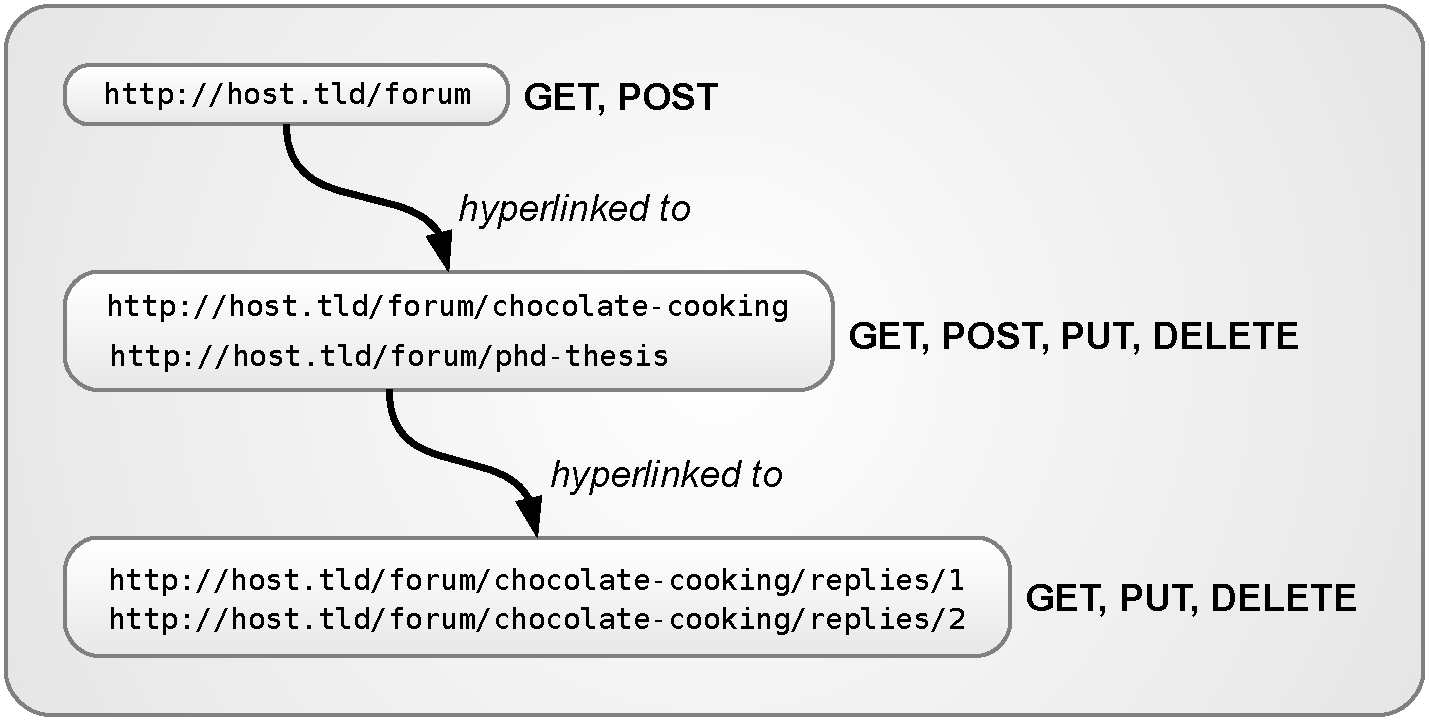
\includegraphics[width=\textwidth]{content/web-services/restful-forum}
    \caption{A \emph{RESTful} forum application.} 
    \label{fig:rest-forum}
\end{figure}

We give an example \emph{RESTful} forum application on Figure~\ref{fig:rest-forum}. It exposes a first resource (\url{http://host.tld/forum}) that supports \emph{GET} and \emph{POST} verbs to fetch the lists of message threads or create a new one. The representation of this resource contains hyperlinks to the resources of the message threads (e.g., \url{http://host.tld/forum/chocolate-cooking}). These resources support all \emph{GET, POST, PUT, DELETE} verbs as a message thread can be asked for its representation (\emph{GET}), a new message can be submitted (\emph{POST}), its title can be updated (\emph{PUT}) and it can be deleted (\emph{DELETE}). Finally, it is also hyperlinked to message replies (e.g., \url{http://host.tld/forum/chocolate-cooking/replies/2}) that can be ``read'', updated or deleted.\\

Two main data representations are used in REST-style web services: XML and JSON (see \url{http://www.json.org/}). JSON is increasingly used as an alternative to XML to represent semi-structured data in web services. It stands for \emph{\textbf{J}ava\textbf{S}cript \textbf{O}bject \textbf{N}otation}. It is basically a textual data exchange format that builds on the \emph{object notation} allowed by the JavaScript language. Indeed, an ``object'' in JavaScript is a associative map between keys and either variables or functions. By combining the former with arrays, a large amount of data can be represented in JSON. We give an example below of the same data first encoded in JSON:
{\footnotesize \verbatiminput{content/web-services/json.txt}}
then in XML:
{\footnotesize \verbatiminput{content/web-services/json-as-xml.txt}}\

The JSON representation is clearly more compact than its XML counterpart (please note that other XML schema could be used to represent this data). While JSON can be used as a general-purpose data representation for data exchange between applications, its main target is web applications (more particularly the so-called AJAX and ``web 2.0'' applications). Indeed, such applications have their client-side logic written in JavaScript as they run in web browsers. By obtaining JSON-encoded data from REST-style services, they can directly use it\footnote{Technically speaking, JavaScript is able to dynamically evaluate code from a string through a function called \texttt{eval}. Web applications can perform an HTTP request to a resource, obtain a JSON-encoded response and use it directly after a call to \texttt{eval}. This is however a serious security weakness as malicious code could be injected in the responses from a compromised server!} since JSON is a fragment of JavaScript. By contrast, XML data is more difficult and time-consuming to parse from JavaScript. Even worse, at the time of this writing the various web browsers vendors have yet to standardize on a JavaScript XML API. There is however a growing consensus over E4X to play this role (see \url{http://www.ecma-international.org/publications/standards/Ecma-357.htm}).\\

REST-style web services offer arguably a higher level of interoperability than SOAP-based ones. The arguments in favor of the REST proponents are generally that:
\begin{enumerate}
  
  \item HTTP libraries are widespread and robust while SOAP libraries are more complex and less mature
  
  \item binding to such services is simpler and it never requires code generation, something which is (too) widespread with SOAP services
  
  \item XML or JSON are well supported by languages and platforms
  
  \item the use of URIs allows for easier and finer-grained monitoring and access filtering of the services, something which is more difficult to do with SOAP endpoints as the message contents need to be looked into.
  
\end{enumerate}\

% ........................................................................... %

\subsection{Syndication services}

% ........................................................................... %

Syndication web services have become increasingly popular with the rise of collaborative online applications such as blogs, wikis and podcasting. They provide resources called \emph{feeds} to notify \emph{subscribers} of events (e.g., a new blog post is available). The service does not directly notifies the subscribers of changes. Rather, it provides a URL-accessible resource which is updated when needed. Subscribers poll this resource for changes on a periodical basis.  There are many types of available clients: web browsers, standalone feed readers, mail clients or aggregating web applications such as \emph{Google Reader} (see \url{http://www.google.com/reader/}).\\

The feed resource representation is usually an XML document for which there are two competing specifications. The first (and historical) one is \emph{RSS} (see \url{http://cyber.law.harvard.edu/rss/rss.html}). RSS stands for \emph{\textbf{R}eally \textbf{S}imple \textbf{S}yndication}, and is based on RDF, the \emph{Resource Description Framework} \cite{DBRG+}. While the first versions were more targeted at news publishing applications, recent versions (especially version 2.0) has been made more versatile. Famous use-cases include audio and video \emph{podcasting} such as supported by media players like \emph{Apple iTunes}. The specifications of RSS have been frozen as of version 2.0 in an attempt to stabilize the RSS ecosystem. RSS is thus closed to further improvements in the near future.\\

The other specification is the \emph{Atom Syndication Format} (see \url{http://www.ietf.org/rfc/rfc4287.txt}) and was first initiated by a group of people who were dissatisfied by RSS. Among the annoyances that had been spotted were a few semantic / ambiguities issues in RSS, the lack of XML namespace use in RSS, the lack of a proper XML schema and the fact that the defining body generally discarded improvement suggestions. Atom is designed to be extensible and open from the ground-up. Better, it has been accepted for standardization by the IETF, and influent companies like Google have made it their official syndication services standard.\\

\begin{figure}[htbp]
    \centering
    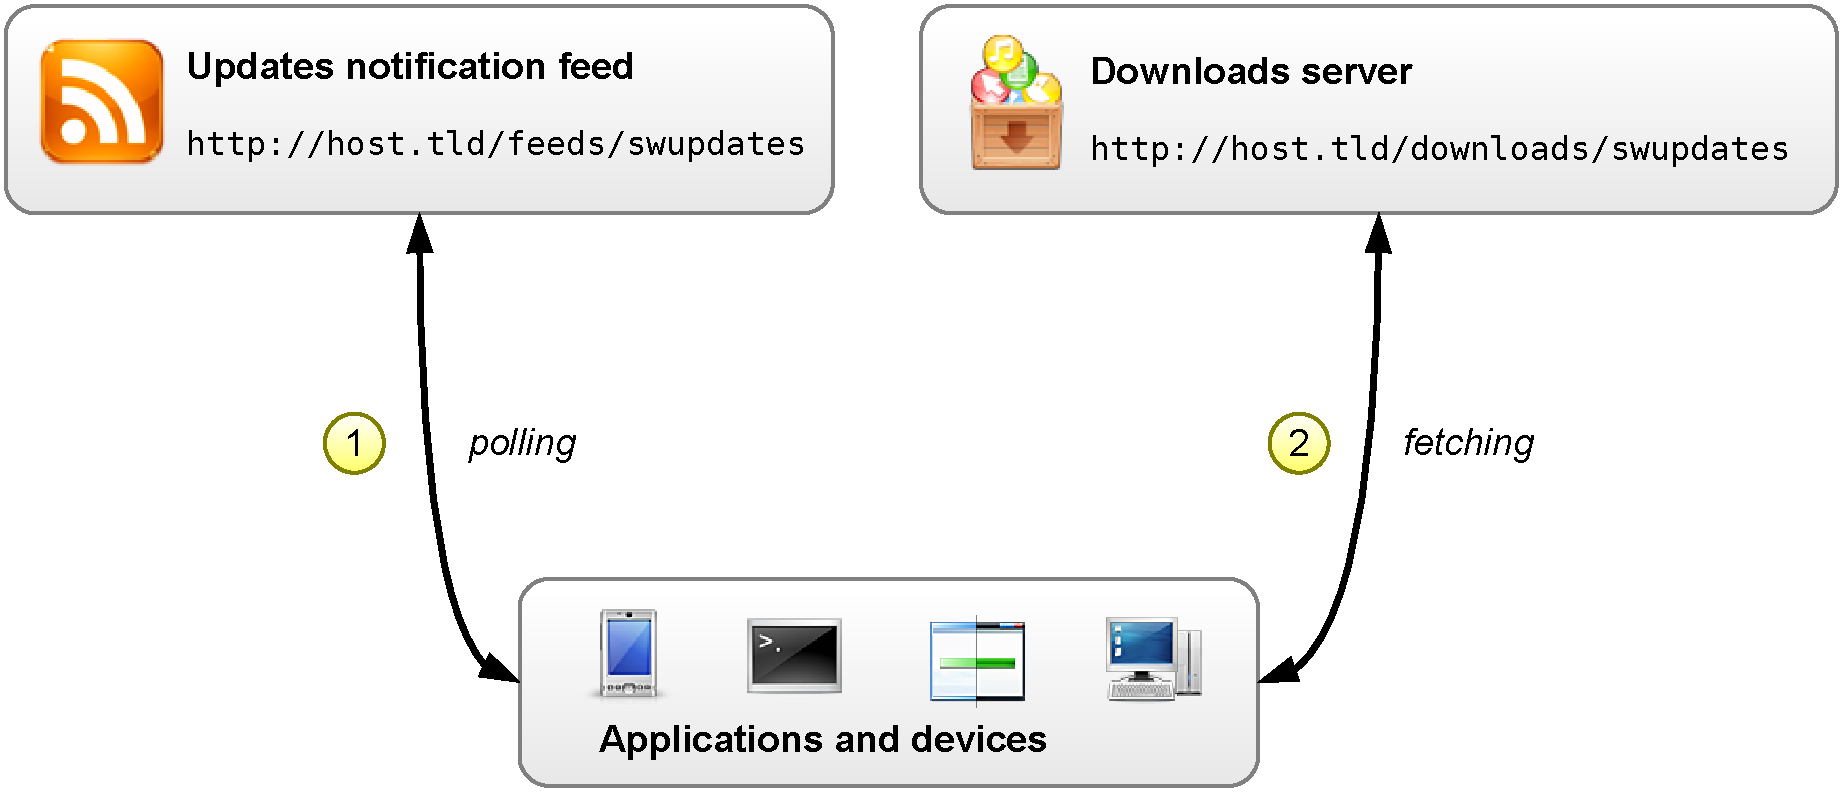
\includegraphics[width=\textwidth]{content/web-services/syndication-scenario}
    \caption{A simple software updates notification and distribution scenario based on syndication.} 
    \label{fig:syndication-scenario}
\end{figure}

While syndication web services have been primarily used for news or content updates, they have many other interesting use-cases when it comes to notifying clients of more ``generic'' event. As an example, consider the scenario depicted on Figure~\ref{fig:syndication-scenario} where a company takes advantage of a syndication web service for providing software updates to the devices used by its employees. A feed is accessible from a URL and the software updates are made available on a dedicated server. Each device owns a small software that is in charge of polling the feed every hour. In case there is an update of a software currently installed on the device, it is be downloaded from the updates server, then installed on the device. To do that, the feed entries provide the URL of the update to download and install. By taking advantage of Atom, such a company could also extend the specification with its own XML namespace, for example to specify the update importance level (ex: critical, normal, minor, ...) and give a chance to the device user to delay the update installation so that ongoing work can be finished first.\\

% ........................................................................... %

\subsection{Comparison}

% ........................................................................... %

\begin{table}[htbp]
\footnotesize
\centering
\begin{tabular}{|p{2.6cm}|p{2.1cm}|p{2.1cm}|p{2.1cm}|p{2.1cm}|}
  
  \hline
  
  -- &
  \textbf{SOAP} &
  \textbf{REST} &
  \textbf{XML-RPC} &
  \textbf{Syndication} \\
  
  \hline
  
  \textit{Target clients} &
  Server-side applications and desktop applications &
  Any &
  Server-side and desktop applications &
  Server-side and desktop applications \\
  
  \hline
  
  \textit{Message exchange patterns} &
  Any &
  Request / response &
  Request / response &
  Publish \& subscribe \\
  
  \hline
  
  \textit{Security} &
  End-to-end &
  Point-to-point &
  Point-to-point &
  Point-to-point \\
  
  \hline
  
  \textit{Binary data support} &
  Very weak &
  Excellent &
  Very weak &
  None (except through hyperlinks) \\
  
  \hline
  
\end{tabular}
\caption{Comparison of the main web services technologies.}
\label{tab:ws-techno-comparison}
\end{table}

We provide in Table~\ref{tab:ws-techno-comparison} a comparison of the web services technologies that we presented above. To do that, we select the following criteria:
\begin{itemize}

	\item the favorite types of client applications for the technology
	
	\item the supported message exchange patterns
	
	\item the level of built-in security to ensure data integrity and confidentiality
	
	\item the level of support for binary data.

\end{itemize}\

Most technologies target server-side and desktop applications as their preferred clients. REST has an advantage here as the possibility to use JSON encoding allows it to be directly used in \emph{rich internet applications} (AJAX, Adobe Flex, Microsoft Silverlight, Mozilla XUL, ...), and HTTP support is ubiquitous. SOAP has the most flexible message exchange patterns support whereas REST and XML-RPC only allow request / response types of interactions between requesters and a service interface. SOAP is also the only solution to support end-to-end security through WS-Security. Point-to-point security (e.g., SSL and HTTPS) is often sufficient in practice as application-encoding of the transported data can still be done (e.g., Java Security API, XML-Encryption, ...). Finally REST has the best support for binary data as HTTP servers and clients support this natively. Encoding binary data in SOAP is difficult (SOAP with attachments) and tied to a single transport channel (HTTP). The other solution (which also applies to XML-RPC) is to encode the binary data using \texttt{base64}, but this is a workaround that can have a significant impact on the XML parsing phases of the transported data. Finally syndication services do not directly transport data (e.g., podcasting services use hyperlinks rather than directly putting the data along with the feed).\\

% ........................................................................... %

\section{SOA: services-oriented architectures}

% ........................................................................... %

We now give an outlook of service-oriented architectures which heavily rely on using web service interfaces. We also give an outlook of service compositions as well as the notions of orchestration and choreography.\\

% ........................................................................... %

\subsection{Overview}

% ........................................................................... %

Service-oriented architectures (SOA) form the new wave of information systems \cite{PTDL07,PH07}. The key idea of SOA is to turn the data sources and applications of an enterprise system into ``small''  distributed units referred to as \emph{services}. Each service is self-encapsulated and it is expected to fulfill a very focused set of coarse-grained functionality requirements (e.g., a payroll processing service is not expected to also handle warehouse provisioning). They can then be assembled to realize applications and business processes. Services provide standard-based, platform-neutral interfaces that hide the implementation details. Also, the services should be autonomous with little dependencies to each other. This means that SOA promotes the loose coupling of services that are used for performing application integration of heterogeneous assets. The loose-coupling comes from both the fact that services are autonomous and that they use open standards for their external access (interfaces and data exchange formats).\\

While approaches with similar goals had been developed before the advent of web services (e.g., Corba, distributed components, ...), they bring some novelty. SOA are indeed often associated with web services as the core mean to realize them. Instead of re-inventing new interface specifications and data encoding means, they directly use widespread, ubiquitous standards such as XML or HTTP. The entry ticket to those technologies is rather low compared to previous approaches, which makes it possible to reuse legacy applications, hide their implementation (including the languages and platform choices) and integrate them with other applications also exposed as services. Another significant improvement in terms of application integration is that SOA blur the traditional boundaries of information systems. Indeed, integrating the information systems of different organizations has traditionally been a costly, largely ad-hoc process as information systems rarely rely on the same technological choices (e.g., languages, platforms) and normative choices (e.g., data representation formats, schema). Technologies such as web services naturally cross networks without having to develop network bridges (e.g., virtual private networks) and as such, they make it ``natural'' to integrate the heterogeneous information systems of different organizations.\\

% ........................................................................... %

\subsection{Orchestration and choreography}

% ........................................................................... %

Those two terms deal with the composition of services in service-oriented architectures. The ability to combine different services (some of them being in-house while others are hosted externally of the organization boundaries) is indeed a key benefit of such loosely-coupled architectures. A composition of services can be viewed as a realization of a business process. Orchestration and choreography allow to describe such processes with the difference between them essentially lying in a difference of point of view.\\

Orchestration focuses on describing the composition from the point of view of an \emph{orchestrator}, i.e., a centralized entity that interacts with each service to realize the composition business process. Orchestration generally relies on workflow-style languages that capture an executable business process. The major orchestration language specification is \emph{BPEL}, the \emph{Business Process Execution Language} (see \url{http://docs.oasis-open.org/wsbpel/2.0/OS/wsbpel-v2.0-OS.html}). Based on XML, this language is able to orchestrate SOAP-based services  by featuring:
\begin{itemize}
  
  \item SOAP service operation calls
  
  \item simple structured constructs (tests, loops) and parallel branches execution
  
  \item data manipulation based on XPath queries with extensions
  
  \item asynchronous interactions with services allowed by a message correlation mechanism
  
  \item support for long-running transactions.
  
\end{itemize}
Last but not least, BPEL exposes process as SOAP services which can in turn be re-used in other compositions. Lesser-known alternatives to BPEL include YAWL \cite{AalstADH04,AalstH05}, a general-purpose workflow language that has support for web services.\\

Choreography focuses on describing the valid message exchanges between services to realize a business process. As such, it ``observes'' the peer-to-peer interactions between the services that take part in a composition. A choreography is generally not executable. WS-CDL (see \url{http://www.w3.org/TR/ws-cdl-10/}) is the reference specification in this area. Tools leveraging WS-CDL are emerging \cite{KangWH07}.\\

\begin{figure}[htbp]
    \centering
    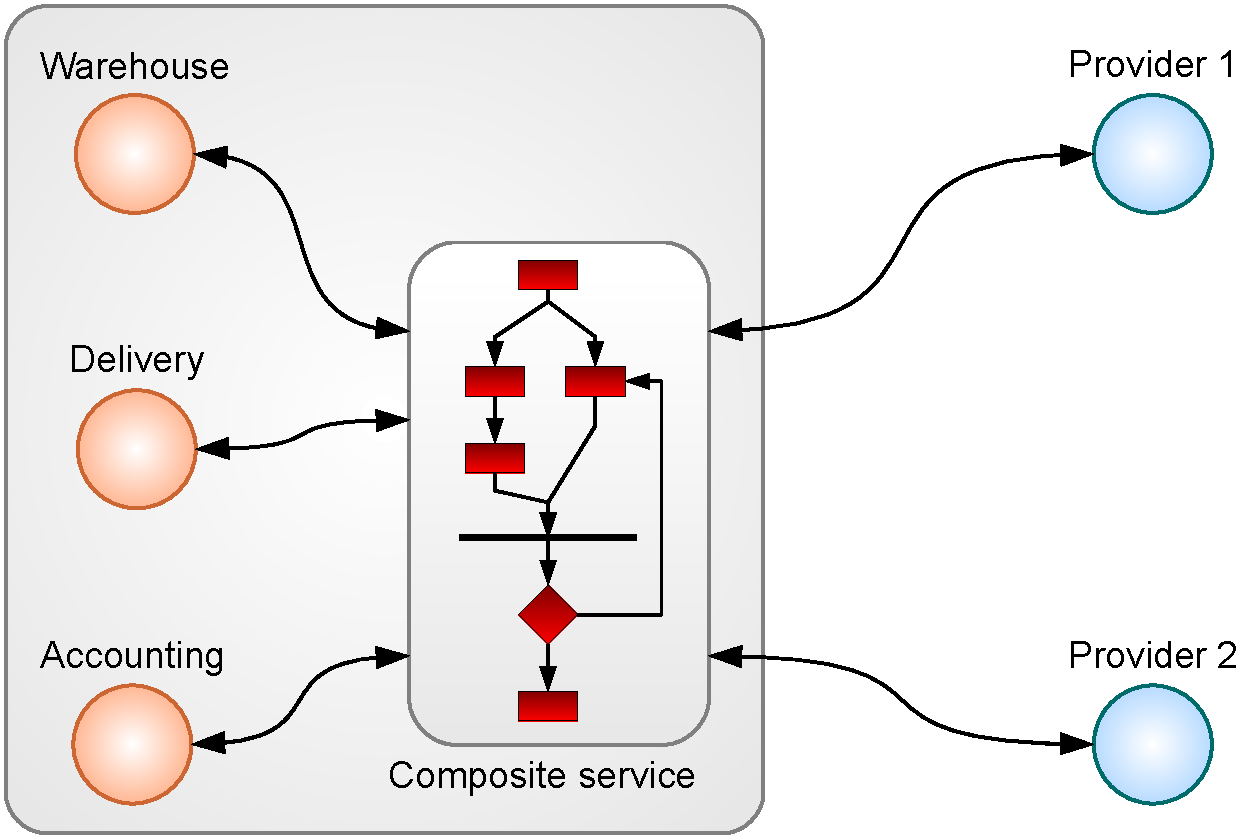
\includegraphics[width=\textwidth]{content/web-services/soa-composition-scenario}
    \caption{A SOA composition scenario.}
    \label{fig:soa-composition-scenario}
\end{figure}

We give an example of a simple service-oriented architecture on Figure~\ref{fig:soa-composition-scenario}. Three in-house services are provided: a warehouse management service, a delivery service and an accounting service. Each of them is an interface to larger applications and data sources and may well have been implemented using different technologies. There are also two external services of providers. A composite service is created by using an orchestration described by a BPEL process (which is not detailed on the figure). When a purchase order, it first checks with the warehouse for availability. If not, a quote is asked to each provider for provisioning the warehouse with the cheapest offer. Once this is done, goods are removed from the warehouse for delivery and the payment is delegated to the accounting.\\

This example shows that such autonomous services facilitate architecting the information by re-using new and legacy applications exposed through standard-based interfaces. The composition of the services allows for proper layering of the service artifacts. The opposite approach would be to allow direct peer-to-peer interactions between the services (e.g., the warehouse service asks for quotation to the provider itself) but as in traditional application integration, this leads to a higher complexity as it gets harder to maintain in the long term (this is also sometimes called the ``spaghetti syndrome''). By contrast, it is possible in this example to externalize the accounting of the organization very quickly: all that is needed is that the accounting provider offers a service with a compatible interface (or more realistically with minimal adaptation required). This is by itself a significant improvement over the previous organization-to-organization integration techniques. \\

% ........................................................................... %
